\section{Global System View}
%
%The proposed system consists of a Graphical User Interface (GUI) that will be on a laptop and up to five 7.5cm spheres.  Figure~\ref{fig:GSV1} shows an idea of how experiments will be conducted by researchers using this system.  As it shows, they will have a laptop with the necessary hardware and software on a jet ski and at least one sphere to throw into the water.  Their current experimental setup allows for a computer to reside on the jet ski they use to deploy the spheres without risking water damage.
%
%\begin{figure}[H]
%	\centering
%	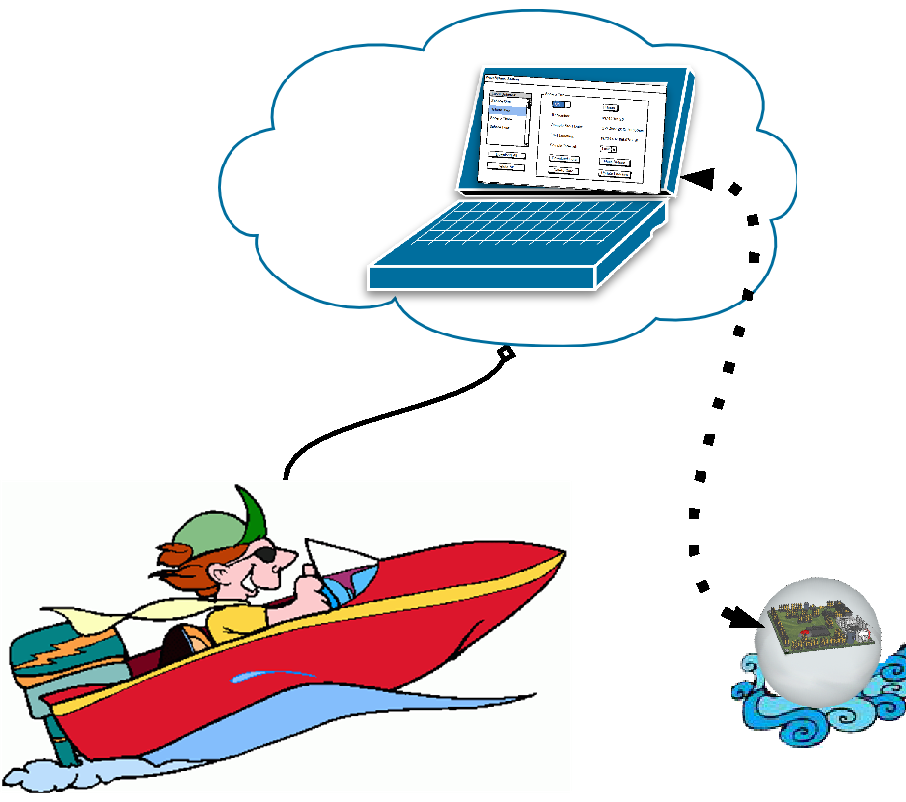
\includegraphics[scale=0.5]{img/GSV1}
%	\caption{Experimental Setup. \label{fig:GSV1}}
%\end{figure}
%
%Figure~\ref{fig:GSV1} shows the interaction between the computer and one sphere, which is the scope of this project, yet the base will be able to handle more than one sphere.  Figure~\ref{fig:GSV2} shows how the interaction would be between multiple spheres, in this case four, and the laptop base station.  The base station should have the capability of connecting with multiple spheres and working with them individually.



The proposed system consists of a Graphical User Interface (GUI) that will be on a laptop and up to five 7.5cm spheres.  Figure~\ref{fig:GSV2} shows an idea of how experiments will be conducted by researchers using this system.  As it shows, they will have a laptop with the necessary hardware and software on a jet ski and at least one sphere to throw into the water.  Their current experimental setup allows for a computer to reside on the jet ski they use to deploy the spheres without risking water damage.  Although this project will focus on building only one sphere, the base station will be able to handle multiple spheres, at least five, at once.  The base station should have the capability of connecting with multiple spheres and working with them individually.

\begin{figure}[H]
	\centering
	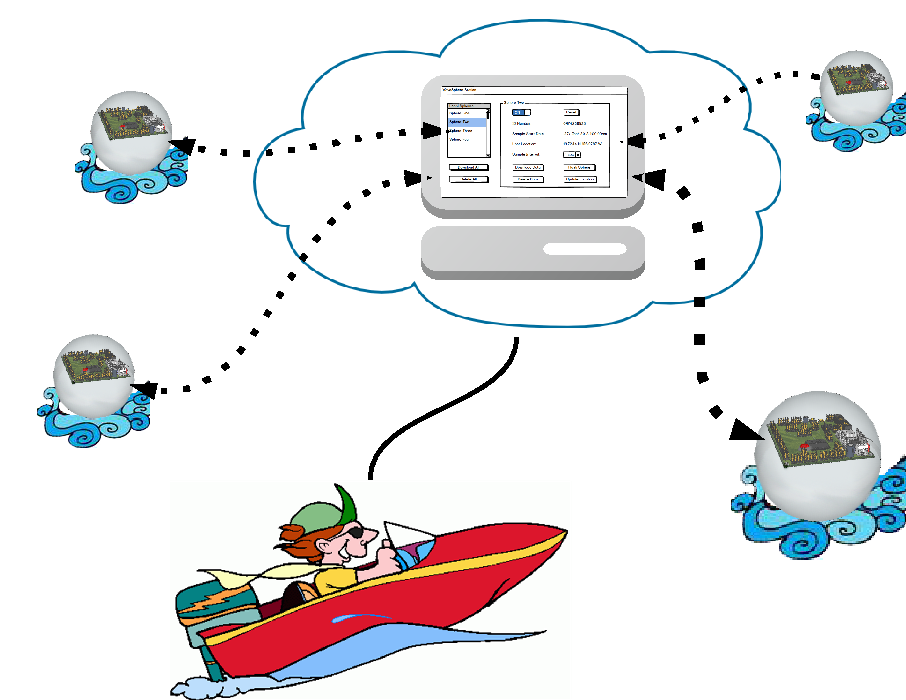
\includegraphics[scale=0.6]{img/GSV2}
	\caption{A rough model of the interaction between the base and multiple spheres. \label{fig:GSV2}}
\end{figure}

Figure~\ref{fig:GSV3} gives a closer look to the interaction between spheres and the base station software.  It shows a software prototype that will be in charge of controlling the necessary hardware in order to communicate with the spheres and perform the necessary tasks such as transfer data from spheres, locate a sphere, reset a sphere or turn off a sphere.  Note that this is a GUI prototype and might be missing some functionality that will form part of this project final system software.  

\begin{figure}[H]
	\centering
	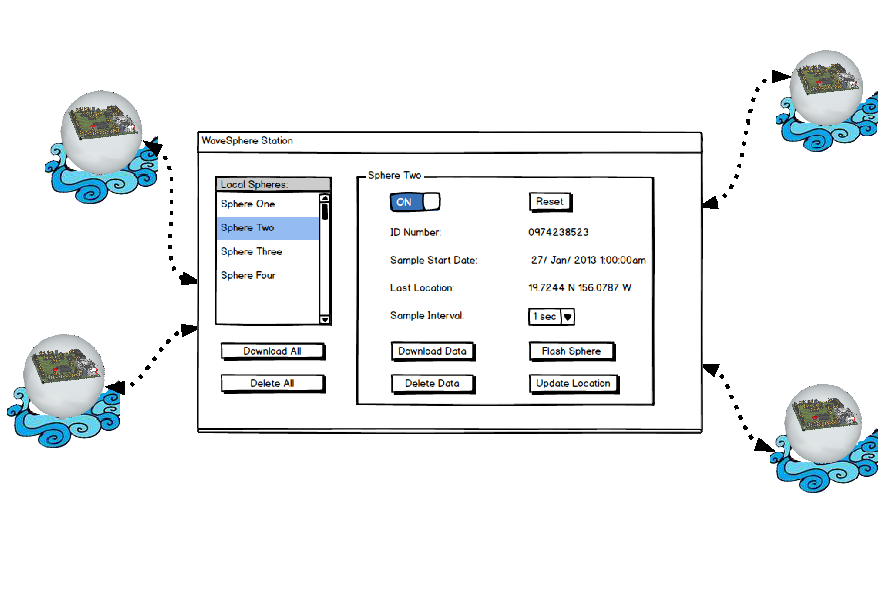
\includegraphics[width=0.9\textwidth]{img/GSV3}
	\caption{A closer look at the interaction between the base and the spheres. \label{fig:GSV3}}
\end{figure}

Finally, Figure~\ref{fig:sphere} shows the concept how the sphere will look like.  A PCB board containing all the necessary hardware will be located axisymmetrically inside the sphere.  This board will be adhered to the sphere such that the hardware does not move freely inside the sphere during the experiments.  Internal designs for mounting components inside the sphere are still being developed and considered as they depend highly on the battery charging methods described in Section~\ref{sec:chargingMethods}.

\begin{figure}[H]
	\centering
	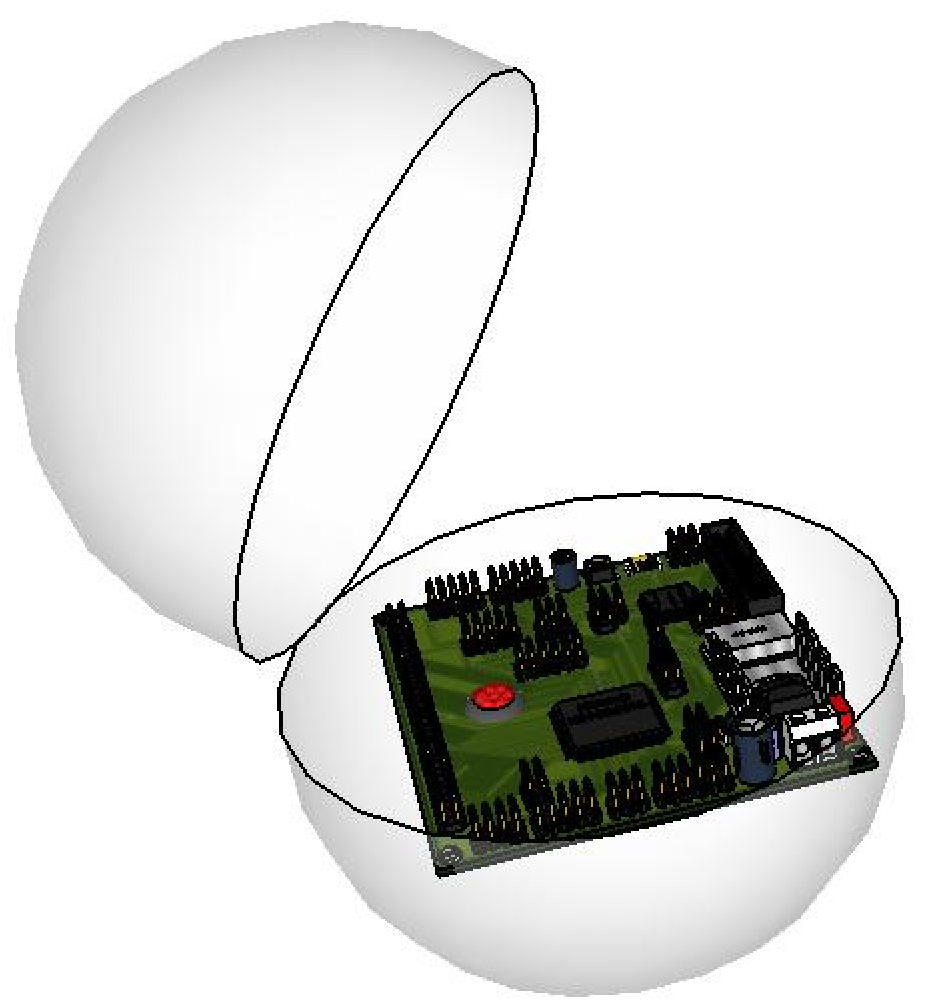
\includegraphics[scale=0.6]{img/Sphere_001}
	\caption{Rough model of hardware inside the sphere. \label{fig:sphere}}
\end{figure}
